%https://tex.stackexchange.com/questions/37581/latex-figures-side-by-side
% put a double figure side by side

%\documentclass[12pt]{report}
%\documentclass[12pt]{extreport}
\documentclass[14pt]{extarticle}
%\documentclass{memoir}

\usepackage{graphicx}
\usepackage{setspace}
\usepackage{amsmath,amssymb}
\usepackage{IEEEtrantools}
\usepackage{cancel}
\usepackage[font=small,labelfont=bf]{caption}
\usepackage{subcaption}
\usepackage{enumitem}

\usepackage{verbatim}
%\usepackage{textcomp}
\usepackage{eurosym}


\usepackage[T1]{fontenc}
\usepackage[utf8]{inputenc}
\usepackage[italian]{babel}


%\usepackage{imakeidx}%
%\makeindex[program=xindy]%, options=-C utf8 -L portuguese]%
\usepackage{makeidx}
\makeindex

\usepackage{enumitem}


\usepackage{geometry}
 \geometry{
 a4paper,
 total={170mm,264mm},
 left=8mm,
 right=8mm,
 top=20mm,
 bottom=10mm
 }









%\renewcommand\thesubsection{\alph{subsection})}


\begin{document}

%\backmatter
%text\index{test}
%\printindex

\pagenumbering{gobble}

\begin{center}
{\bf Compito in classe di matematica}
\end{center}



\begin{enumerate}[label=\bfseries\arabic*)]
	\item Calcola il M.C.D. e il m.c.m. fra le espressioni dei seguenti gruppi.
		\begin{enumerate}
			\item
				$
					45;\qquad 64;\qquad 40
				$
			\item
				$
					6ab^3c^2;\qquad 14a^2bc^4			
				$				
			\item
				$
					18xy^3; \qquad 60x^2yz; \qquad 30 x^2y			
				$
		\end{enumerate}
	
	\item Scomponi i seguenti polinomi in fattori primi. 

	\vspace{-10pt}

	{\tiny (gli eventuali monomi simili vanno sommati)}
	
		\begin{enumerate}
			
			\item[] raccoglimento TOTALE 
			\item
				$
					-2a^3b^4 + a^2b^3
				$
			\item
				$
					30a^3b^2c^4 - 12a^4b^3c^3 + 24a^2bc^5 
				$
			\item
				$
					a\left( a + b \right) - 2\left( a + b \right)
				$			
			\item
				$
					\left( x + 1 \right)\left( x^2 + 1 \right) - \left( x - 1 \right)\left( x^2 + 1 \right)
				$


			\item[] raccoglimento PARZIALE 
			
			\item 
					$
						2a^3 + a^2b + 2ab^2 + b^3
					$


		\end{enumerate}
	
		\item Eseguire le seguenti somme tra frazioni
			\begin{enumerate}
				\item
					$
						\frac{7}{90} - \frac{11}{75}
					$				
				\item
					$
						\frac{5x}{2x^2 - 4x} - \frac{1}{3x - 6}
					$
			\end{enumerate}
		
		\item Risolvere le seguenti equazioni:
		\begin{enumerate}
			\item 
				$
					2 + 2\left( 7 - 3x \right) + x = 5 -3(5 - x)
				$
			\item 
				$
					(x - 3)(x+3) - (x + 2)^2 + x = 0
				$
		\end{enumerate}
		\item Al negozio acquisto una bicicletta, il suo prezzo pieno è di $450$ euro e viene scontata del $20\%$
		




		\begin{figure}[h]
		    \begin{minipage}{0.6\textwidth}
				\begin{enumerate}
			    		\item Calcolare a quanto ammonta lo sconto;
			    		\item Calcolare a quanto ammonta il costo effettivo della bicicletta;
			    		\item Del costo effettivo della bicicletta, soltanto i 2/5 li pago di tasca mia, il resto li paga la mia mamma. Calcolare quanto pago io quanto paga la mamma.
				\end{enumerate}
		    \end{minipage}
		    \hfill
		    \begin{minipage}{0.3\textwidth}
				\centering
				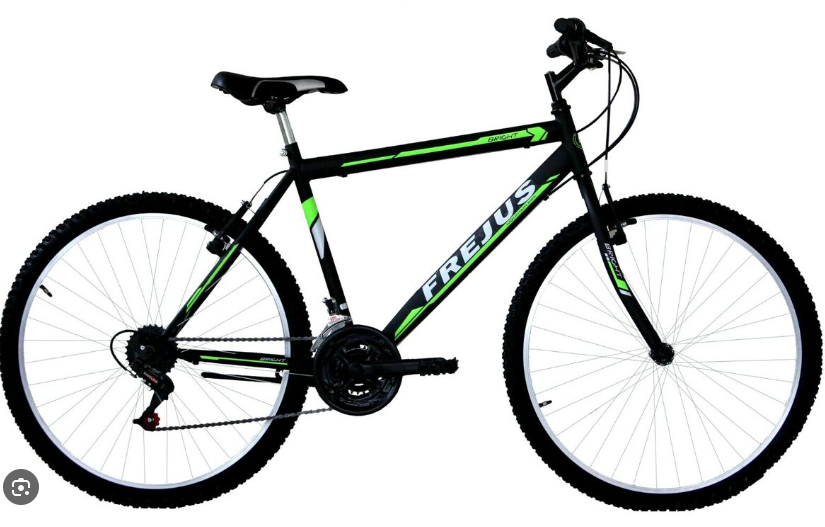
\includegraphics[width=\textwidth]{bicicletta.png} % Replace "bicicletta.png" with your image file
				%\caption{Didascalia dell'immagine}
		    \end{minipage}
		\end{figure}






\end{enumerate}



\newpage

\begin{center}
{\bf Compito in classe di matematica}
\end{center}

\begin{enumerate}[label=\bfseries\arabic*)]
	\item Calcola il M.C.D. e il m.c.m. fra le espressioni dei seguenti gruppi.
		\begin{enumerate}
			\item
				$
					90;\qquad 32;\qquad 80
				$
			\item
				$
					14a^2bc^3;\qquad 6ab^3c^2			
				$				
			\item
				$
					60x^2yz; \qquad 18xy^3; \qquad 30 xy^2			
				$
		\end{enumerate}
	
	\item Scomponi i seguenti polinomi in fattori primi.
	
	\vspace{-10pt}

	{\tiny (gli eventuali monomi simili vanno sommati)}
	
		\begin{enumerate}
			
			\item[] raccoglimento TOTALE 
			\item
				$
					a^2b^3 -2a^3b^4
				$
			\item
				$
					12a^4b^3c^3 - 30a^3b^2c^4 + 36a^2bc^3 
				$
			\item
				$
					8\left( a + b \right) - x\left( a + b \right)
				$			
			\item
				$
					- \left( a - 1 \right)\left( a^2 + 1 \right) + \left( a + 1 \right)\left( a^2 + 1 \right)
				$


			\item[] raccoglimento PARZIALE 
			
			\item 
					$
						2ab^2 + b^3 + 2a^3 + a^2b
					$


		\end{enumerate}
	
		\item Eseguire le seguenti somme tra frazioni
			\begin{enumerate}
				\item
					$
						\frac{13}{90} - \frac{7}{75}
					$				
				\item
					$
						\frac{1}{5x - 10} - \frac{5x}{2x^2 - 4x}
					$
			\end{enumerate}
		
		\item Risolvere le seguenti equazioni:
		\begin{enumerate}
			\item 
				$
					5 -3(5 - x) = 2 + 2\left( 7 - 3x \right) + x
				$
			\item 
				$
					(x + 2)^2 - (x - 3)(x+3) = x
				$
		\end{enumerate}
		
		
		




		\item Al negozio acquisto una bicicletta, il suo prezzo pieno è di $900$ euro e viene scontata del $15\%$
		




		\begin{figure}[h]
		    \begin{minipage}{0.6\textwidth}
				\begin{enumerate}
			    		\item Calcolare a quanto ammonta lo sconto;
			    		\item Calcolare a quanto ammonta il costo effettivo della bicicletta;
			    		\item Del costo effettivo della bicicletta, soltanto i $2/5$ li pago di tasca mia, il resto li paga la mia mamma. Calcolare quanto pago io quanto paga la mamma.
				\end{enumerate}
		    \end{minipage}
		    \hfill
		    \begin{minipage}{0.3\textwidth}
				\centering
				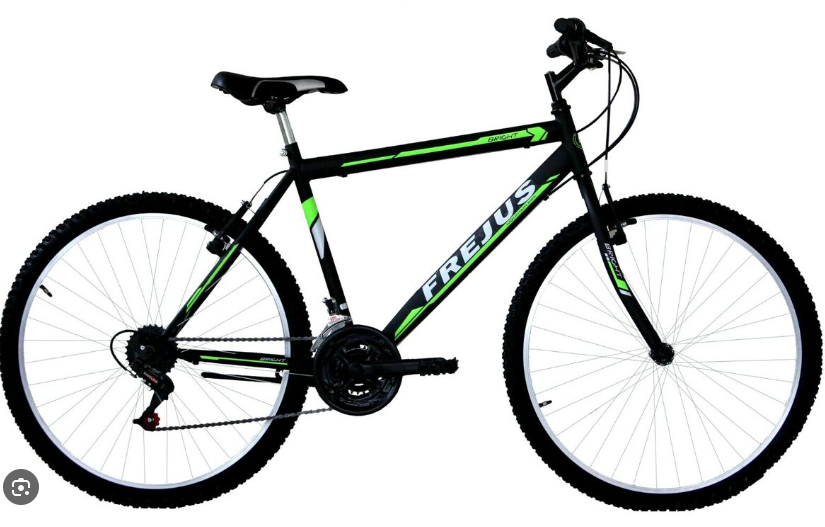
\includegraphics[width=\textwidth]{bicicletta.png} % Replace "bicicletta.png" with your image file
				%\caption{Didascalia dell'immagine}
		    \end{minipage}
		\end{figure}





\end{enumerate}


\newpage


\begin{center}
{\bf Compito in classe di matematica}

{\tiny E' consentito l'uso della calcolatrice}
\end{center}


\begin{enumerate}[label=\bfseries\arabic*)]
	\item Calcola il M.C.D. e il m.c.m. fra le espressioni dei seguenti gruppi.
		\begin{enumerate}
			\item
				$
					45;\qquad 64;\qquad 40
				$
			\item
				$
					6ab^3c^2;\qquad 14a^2bc^4			
				$				
			%\item
			%	$
			%		18xy^3; \qquad 60x^2yz; \qquad 30 x^2y			
			%	$
		\end{enumerate}
	
	\item Scomponi i seguenti polinomi in fattori primi. 

	\vspace{-10pt}

	{\tiny (gli eventuali monomi simili vanno sommati)}
	
		\begin{enumerate}
			
			\item[] raccoglimento TOTALE 
			\item
				$
					-2a^3 + a^2
				$
			\item
				$
					3a^3b - 12ab^3c + 6ab 
				$
			\item
				$
					x\left( y + z \right) - 2\left( y + z \right)
				$			
			\item
				$
					\left( a + 1 \right)\left( a^2 + 1 \right) - \left( a - 1 \right)\left( a^2 + 1 \right)
				$


			\item[] raccoglimento PARZIALE 
			
			\item 
					$
						2a^3 + a^2b + 2ab^2 + b^3
					$


		\end{enumerate}
	
		\item Eseguire le seguenti somme tra frazioni
			\begin{enumerate}
				\item
					$
						\frac{1}{12} - \frac{5}{18}
					$				
				\item
					$
						\frac{5x}{2x^2 - 4x} - \frac{1}{3(x - 2)}
					$
			\end{enumerate}
		
		\item Risolvere le seguenti equazioni:
		\begin{enumerate}
			\item 
				$
					14 - 6x + x = 5 -3(5 - x)
				$
			\item 
				$
					(x + 2)^2 = x^2
				$
		\end{enumerate}
		
		
		\item Al negozio acquisto una bicicletta, il suo prezzo pieno è di $450$ euro e viene scontata del $10\%$
		




		\begin{figure}[h]
		    \begin{minipage}{0.6\textwidth}
				\begin{enumerate}
			    		\item Calcolare a quanto ammonta lo sconto;
			    		\item Calcolare a quanto ammonta il costo effettivo della bicicletta;
			    		\item Del costo effettivo della bicicletta, soltanto $1/3$ li pago di tasca mia, il resto li paga la mia mamma. Calcolare quanto pago io quanto paga la mamma.
				\end{enumerate}
		    \end{minipage}
		    \hfill
		    \begin{minipage}{0.3\textwidth}
				\centering
				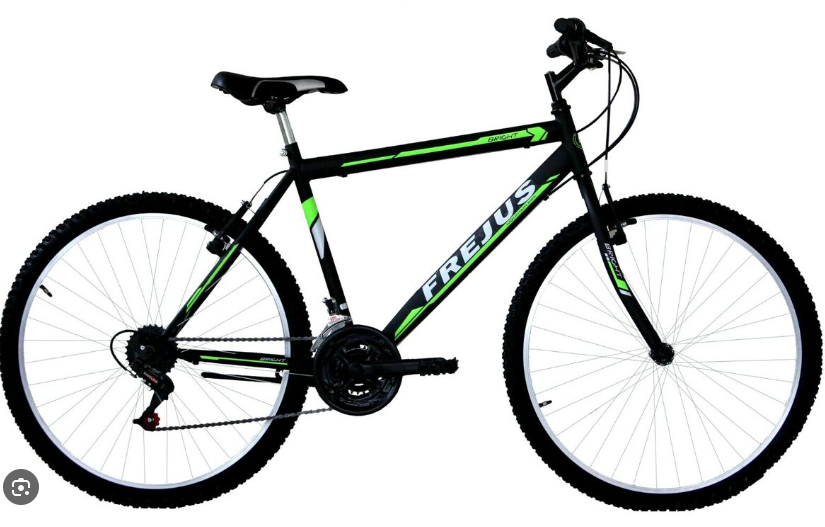
\includegraphics[width=\textwidth]{bicicletta.png} % Replace "bicicletta.png" with your image file
				%\caption{Didascalia dell'immagine}
		    \end{minipage}
		\end{figure}


		
		
				

\end{enumerate}



\end{document}